\debut{Emile Martinez}{}{Représentation binaire, graphes}{Tanenbaum, Balabonski 1ère, 2nd SNT Beaude Quenet}

\begin{com}
	On peut ici avoir une discussion sur le terme architecture. L'architecture c'est «Principe d'organisation d'un ensemble, agencement, structure». On peut donc penser à l'architecture physique. On parlerait alors des types de lien, de serveurs, de ou les placés, de qui controle quoi, de la mainère de faire des routeurs, etc. Néanmoins plus proches des notions du programme, on parlera plus ici d'architecture logicielle. Donc l'architecture conceptuelle, les différents protocoles qui s'empilent pour faire fonctionné cela. 
\end{com}

\section{Mise en Contexte}

\subsection{Historique}

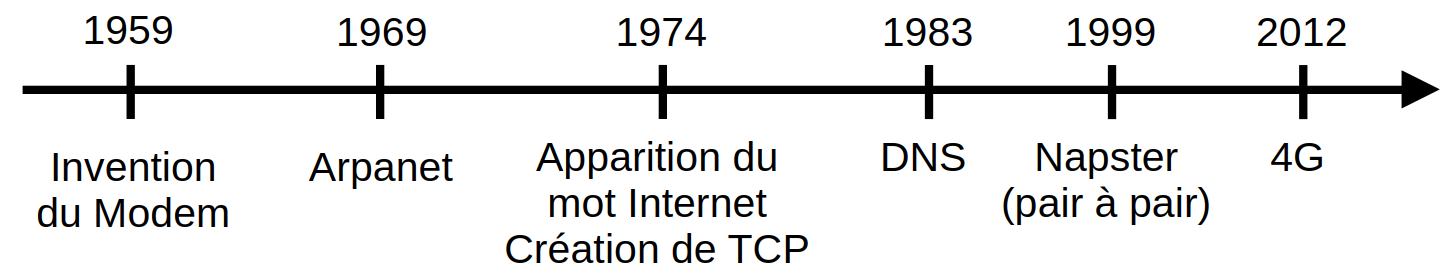
\includegraphics[width=\linewidth]{lecon/26-architecture-internet/frise.png}

\subsection{Maintenant}

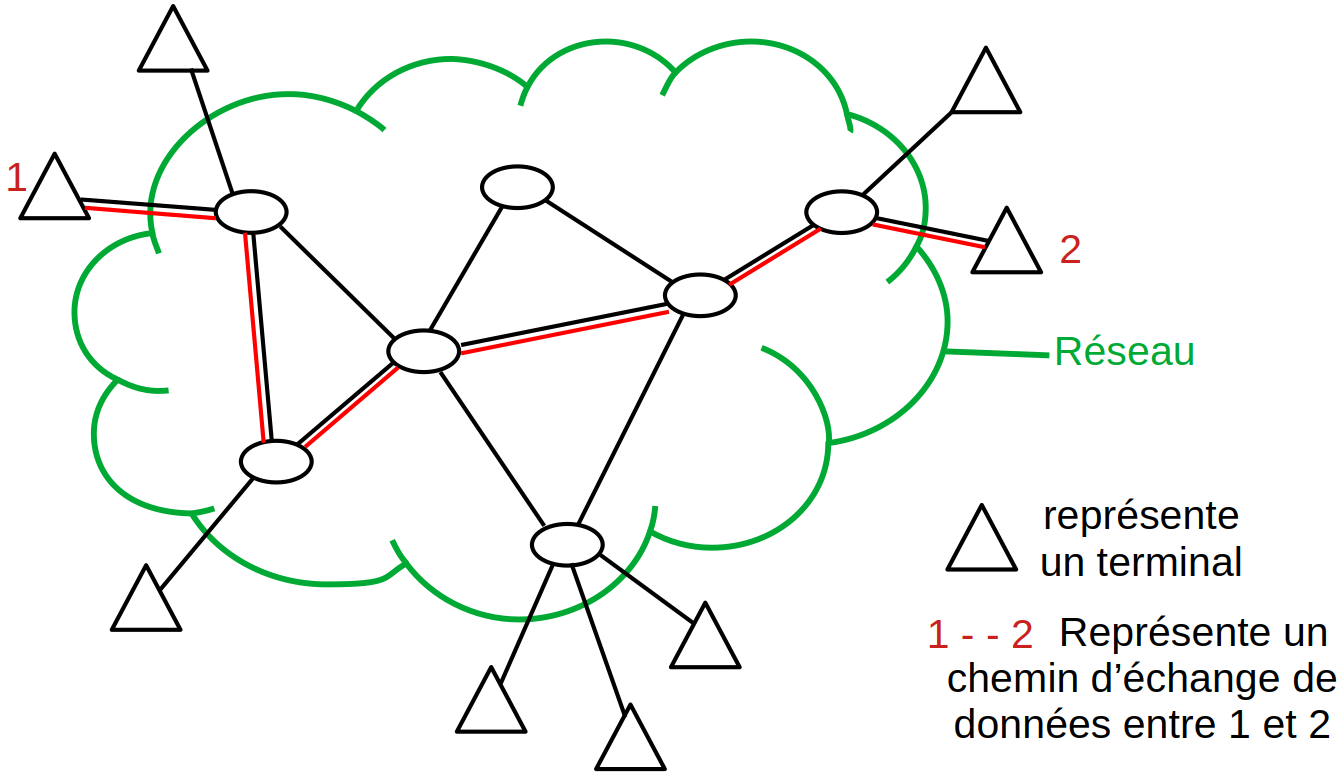
\includegraphics[width=\linewidth]{lecon/26-architecture-internet/chemin_reseau.png}

Désormais, des milliards d'utilisateurs sont connectés à travers l'internet.

\section{Modèles des couches OSI}

Fais le lien entre les besoins d'une application et les messages transitant sur internet

\begin{tabular}{p{0.45\linewidth}:p{0.45\linewidth}}
	\begin{center}
		\textbf{\textcolor{blue}{\underline{Réseau}}}
	\end{center} &
	\begin{center}
	\textbf{\textcolor{blue}{\underline{Poste}}}
	\end{center} \\
	&\\
	
	\begin{minipage}{\linewidth}
		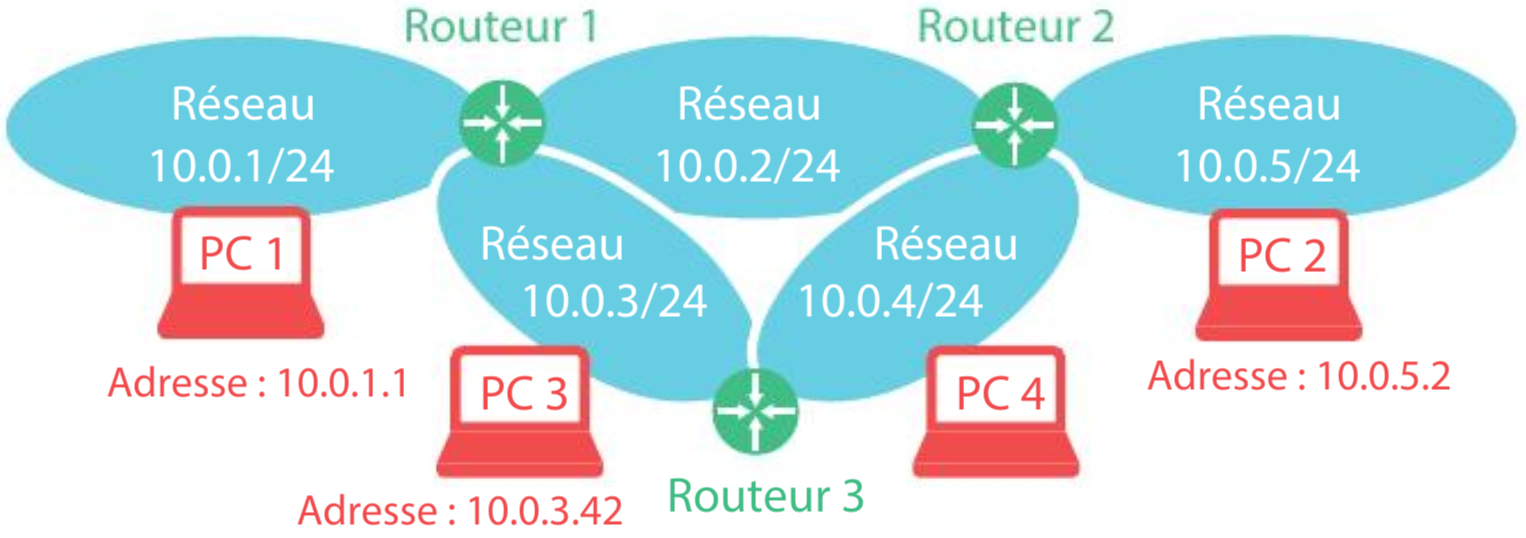
\includegraphics[width=\linewidth]{lecon/26-architecture-internet/schema_osi.png} \\ \\
		(schém honteusement volé de ce livre https://www.mesmanuels.fr/acces-libre/9782278094912)
	\end{minipage} & \raisebox{-0.5\height}{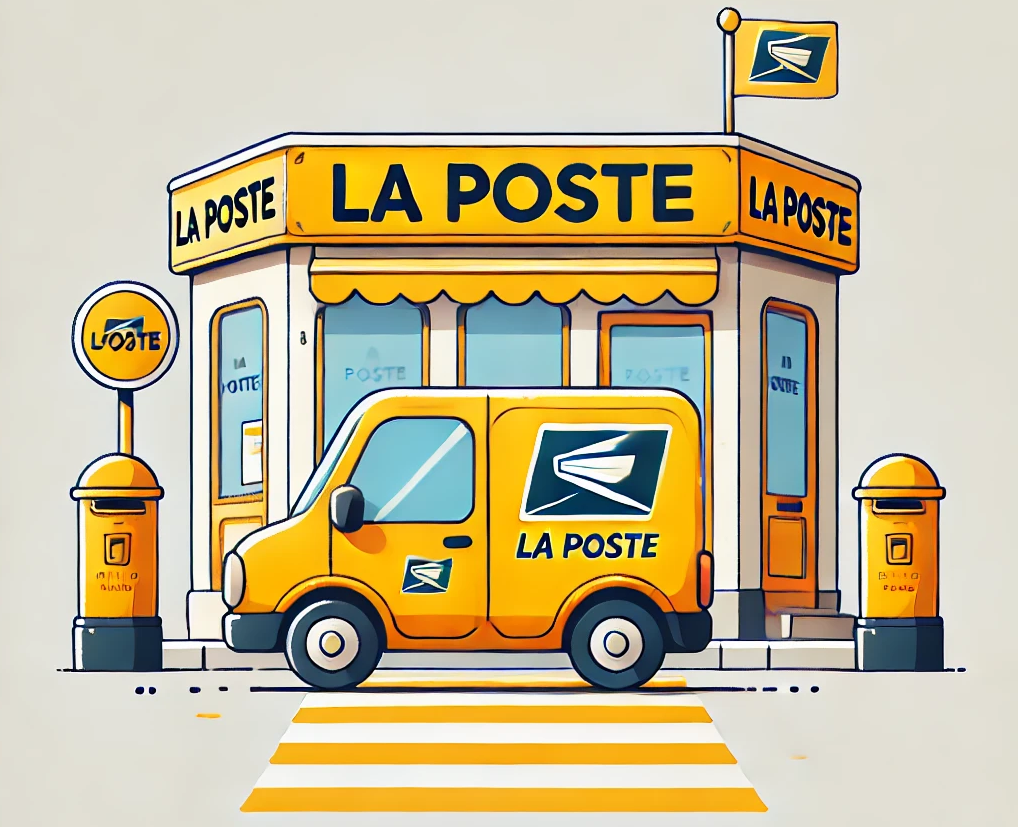
\includegraphics[width=\linewidth]{lecon/26-architecture-internet/poste.png}} \\
	& \\ \hdashline
	
	\multicolumn{2}{c}{\underline{Couche Applicative}} \\
	Fais le lien entre les besoins d'une application et les messages transitant sur internet &
	Manière de lire et écrire une lettre. Langue dans laquelle on comunique \\
	&\\ \hdashline
	
	\multicolumn{2}{c}{\underline{Couche Transport}} \\
	Centralise les données qu'envoient différentes applications d'une même machine et les mets sur le réseau. C'est le lien entre le PC et le réseau & poster le courrier, aller le chercher dans la boite aux lettres, et le repartir entre les différentes habitants \\
	&\\ \hdashline
	
	
	\multicolumn{2}{c}{\underline{Couche Réseau}} \\
	S'occupe de faire passer les données d'un réseau à un autre. C'est là qu'on décide la direction que doit prendre la donnée. C'est ce qu'on appelle le routage. & Centre de tri (ou bureau de poste) mettant en sac postal et donnant le prochain lieu ou doit aller le sac postal \\
	&\\ \hdashline
	
	
	\multicolumn{2}{c}{\underline{Couche Lien}} \\
	Achemine les données à l'intérieur d'un réseau & le kangoo jaune, le train entre deux gare de triage, le porteur qui amène le sac de lettre du quai au wagon postal, etc\dots
\end{tabular}

\begin{rem}
	La structure d'internet est assez indépendante de la technologie sous-jacente. Comme l'organisation de la poste ne dépend que à la marge du véhicule qu'utilise le facteur.
\end{rem}

\begin{personalise}[Conséquence]
	La technologie peut évoluer en conservant le travail des couches supérieures (et même plus généralement entre les couches)
\end{personalise}

\begin{com}
	On parle plus de l’indépendance de la structure physique que des couches entre elles car le programme demande d'insister dessus.
\end{com}

\subsection{Paquets}

\begin{principe}[Principe de segmentation]
	Plutôt que d'envoyer toutes les données d'un seul tenant, on les découpe en plein de paquets plus petits qu'on envoie séparément.
\end{principe}

\begin{personalise}[Intérêts]
	\begin{itemize}
		\item Plusieurs paquets peuvent cohabiter sur un même lien (il est facile de dire qu'on envoie un paquet de chaque application à tour de rôle par exemple)
		
		\item Si un paquet est corrompu ( des données à l'intérieur sont fausses) ou se perd, on est pas obligé de tout renvoyer, on peut ne renvoyer que le morceau abîmée
		
		\item On peut maximiser la redondance des liens du réseau en faisant emprunter plusieurs chemin à différents paquets
	\end{itemize}
\end{personalise}

\begin{principe}[Principe d'encapsulation]
	Chaque protocole ajoute un en-tête à chaque paquet pour échanger de l'information, et considère l'en-tête d'avant comme de la données.\\
	\\
	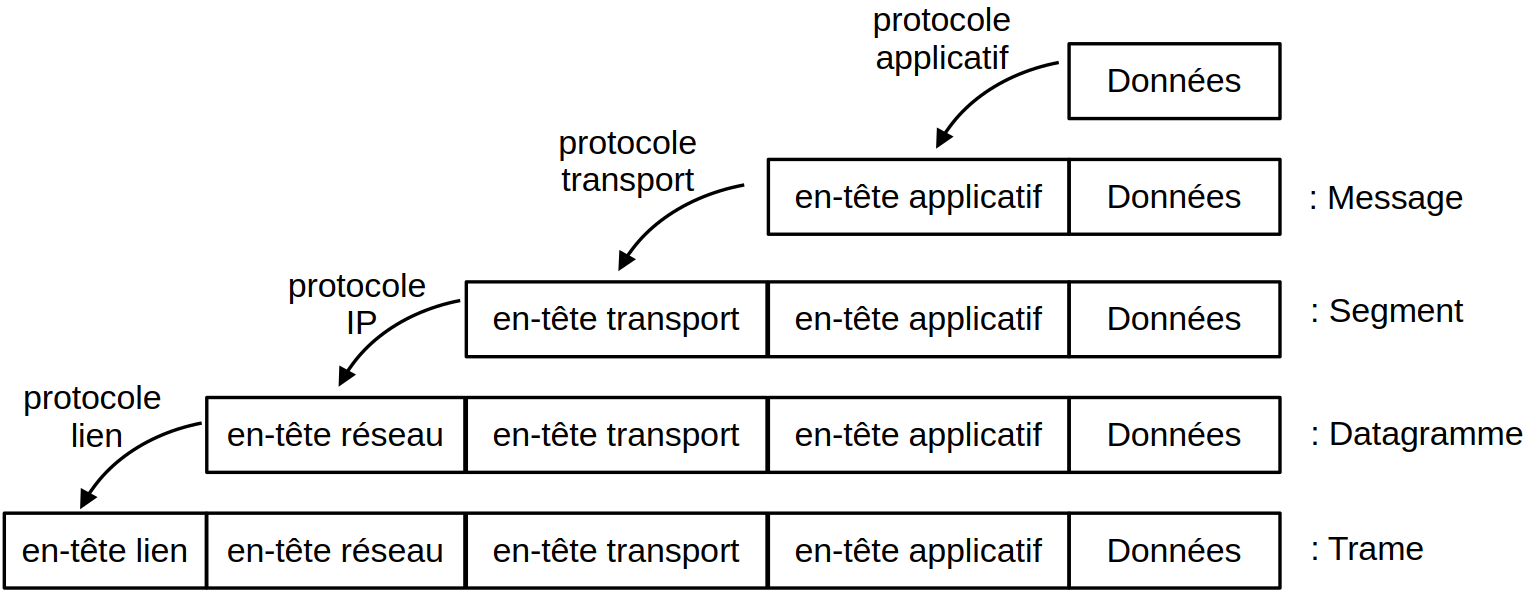
\includegraphics[width=\linewidth]{lecon/26-architecture-internet/encapsulation.png}
\end{principe}

\begin{com}
	Ce schéma pourrait être l'occasion de question avec les élèves, en expliquant plus longuement le principe, puis en leur demandant à leur avis à quelle couche le message est le plus grand (est ce que l'applicatif vient par dessus le transport ou l'inverse). Néanmoins il y a peu de chances qu'ils trouvent. On peut donc éventuellement plutôt le faire, et ensuite poser cette question en devoir.
\end{com}

\subsection{Principe d'un protocole}

\begin{definition}[protocole]
	Un protocole est une manière de faire sur laquelle les différentes parties se mettent d'accord en amont.
\end{definition}

Pour chaque couche et pour chaque chose que l'on veut faire dans cette couche, en réseau, on a des protocoles.

\begin{example}
	Dans l'analgoie de la poste, la manière d'écrire une adresse sur une enveloppe est un protocole  (que l'on pourrait placer à la couche réseau)
\end{example}

\begin{example}
	\begin{itemize}
		\item NTP est un protocole applicatif permettant de syncrhoniser les horologes des ordinateurs
		
		\item FTP est un protocole applicatif permettant d'échanger des fichiers (comme des courriels)
		
		\item UDP est un protocole de la couche transport sans garantie utilisé pour transmettre des flux vidéos
		
		\item DHCP est un protocole de la couche réseau permettant à un nouvel utilisateur d'obtenir une adresse IP
		
		\item Ethernet est un protocole de la couche liaison décrivant comment se transmettre des paquets dans un câble coaxial
	\end{itemize}
\end{example}

\section{Des protocoles structurants}

\subsection{Le protocole IPv4}

C'est un protocole de la couche réseau ayant pour but d'identifier les différents hôtes d'un réseau. Chaque hôte est identifié par un nombre de 32 bits, découpé en  4 nombres de 8 bits :
$$\texttt{1100000010101000000101000101101} \to \texttt{ 11000000.10101000.00010100.00101101} \to \texttt{192.164.10.45}$$

\noindent Paquet IP : \raisebox{-0.5\height}{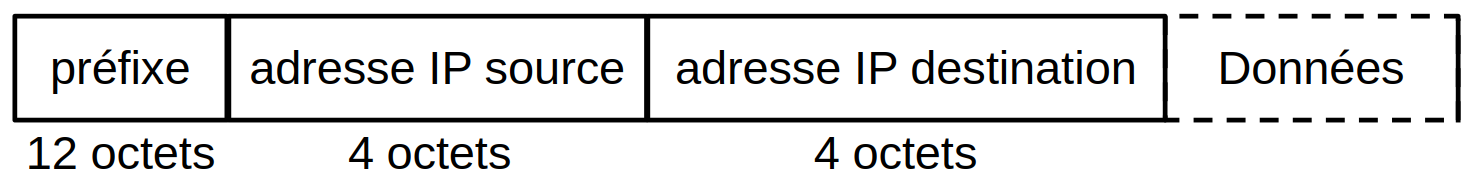
\includegraphics[width=0.7\linewidth]{lecon/26-architecture-internet/paquet_IP.png}}\\

Les routeurs (interfaces entre différents réseaux) garde alors une table de routage dans laquelle à chaque adresse IP est indiqué l'adresse IP du prochain routeur où aller.

\paragraph{Dveloppement :} Convergence de l'algorithme de Bellman-Ford

\begin{personalise}[Problème]
	Les tables sont beaucoup trop grandes
\end{personalise}

\begin{personalise}[Solution]
	Deux machines proches recevront des IPs proches et ainsi on regroupe des machines en sous-réseau, dont les premiers bits des IPs sont les mêmes. Le nombre de bits identiques d'un sous-réseau est indiqué par un nombre après le /x (appelés masque de sous-réseau). Une table de routage n'a alors plus qu'a sauvegarder les sous-réseaux (sauf si il est dans le sous-réseau, où il garderait alors plus)
\end{personalise}

\begin{example}
	\texttt{11000000.11000000.00001010.00101101/20} représente toutes les IP commençant par \texttt{11000000.11000000.0000}
\end{example}

\begin{principe}
	Il arrive que l'on attribue des adresses d'un sous réseau ailleurs. On utilisera alors le principe de correspondance du plus grand préfixe (on va dans le sous réseau valide, où le plus de bits correspondent)
\end{principe}

\begin{rem}
	Dans le champ préfixe on a des informations comme la version du protocole, un code de vérification (pour vérifier que le paquet n'est pas corrompu) ou encore le TTL (time to leave) indiquant le nombre de sauts restants autorisés pour ce paquets (lui évitant de boucler à l'infini).
\end{rem}

\subsection{Le protocole TCP}

Le protocole TCP est un protocole de la couche transport, décidant donc de qui va être envoyé, ré-envoyé, et quand.

\begin{com}
	Si on veut s'étendre sur TCP, on peut reprendre ce qui est fait dans la leçon \ref{L25}, et même éventuellement en récupérer le développement. Néanmoins ça parait moins structurant pour l'architecture globale d'internet.
\end{com}

\begin{principe}
	\begin{itemize}
		\item Offrir des garanties sur les paquets : Pour cela il établit une connexion entre les deux hôtes (par une connexion en trois temps) puis envoie des acquittements pour chaque paquet (pouvant ainsi renvoyer ceux qui ne sont pas arrivés)
		
		\item Réguler le trafic : Pour cela, en fonction de la quantité de paquets perdus ou arrivant en retard, le protocole TCP adapte le taux d'envoi.
	\end{itemize}
\end{principe}

\begin{com}
	On pourrait également dans le premier point rajouter le fait que on peut réordonner les paquets
\end{com}

\subsection{Le protocole DNS}

C'est un protocole de la couche application, parfois appelé «l'annuaire d'internet», qui fait correspondre des adresses IP à des URL lisibles par l'homme. Pour cela, des serveurs répondent l'adresse IP demandée.\\

\begin{minipage}{0.5\linewidth}
	\begin{center}
		\begin{tikzpicture}[-]
			\node[rectangle, draw] (r) {Racine};
			\node[rectangle, draw, below left = 0.5cm and 1cm of r] (fr) {.fr};
			\node[rectangle, draw, below = 0.5cm of r] (com) {.com};
			\node[rectangle, draw, below right = 0.5cm and 1cm of r] (org) {.org};
			\node[rectangle, draw, below = 0.5cm of fr] (wiki) {wikipedia.fr};
			\node[rectangle, draw, below left = 0.5cm and -0.2cm of org] (agreg) {agreg-info.org};
			\node[rectangle, draw, below right = 0.5cm and -0.2cm of org] (w) {wikipedia.org};
			
			\draw (r) edge[] (fr);
			\draw (r) edge[] (com);
			\draw (r) edge[] (org);
			\draw (fr) edge[] (wiki);
			\draw (org) edge[] (agreg);
			\draw (org) edge[] (w);
			
		\end{tikzpicture}
	\end{center}
\end{minipage} \begin{minipage}{0.3\linewidth}
	Pour transformer un URL en adresse IP, on demande alors à chaque serveur l'adresse du serveur suivant.
\end{minipage}\\\\

\begin{personalise}[Schéma][Résolution d'une requête DNS] 
	\begin{center}
		\begin{tikzpicture}
			\node[rectangle, draw, inner sep=0.2cm] (dom) {www.domaine.org};
			\node [rectangle, draw, inner sep=0.2cm, above right = 1cm and 3cm of dom] (r) {Serveur Racine};
			\node [rectangle, draw, inner sep=0.2cm, right = 3cm of dom] (org) {Serveur .org};
			\node [rectangle, draw, inner sep=0.2cm, below right = 1cm and 3cm of dom] (sdom) {Serveur domaine.org};
			
			\draw ([yshift = 0.5cm]dom.east) edge[->, above left] node{1} ([yshift = 0.1cm]r.west);
			\draw ([yshift = 0.3cm]dom.east) edge[<-, below left] node{2} ([yshift = -0.1cm]r.west);
			\draw ([yshift = 0.1cm]dom.east) edge[->, above right] node{3} ([yshift = 0.1cm]org.west);
			\draw ([yshift = -0.1cm]dom.east) edge[<-, below right] node{4} ([yshift = -0.1cm]org.west);
			\draw ([yshift = -0.3cm]dom.east) edge[->, above left] node{5} ([yshift = 0.1cm]sdom.west);
			\draw ([yshift = -0.5cm]dom.east) edge[<-, below left] node{6} ([yshift = -0.1cm]sdom.west);
			
		\end{tikzpicture}
	\end{center}
\end{personalise}

\subsection{HTTP}

C'est un protocole omniprésent de la couche application. Il sert à échanger des pages web.\\

Son en-tête contient des informations comme le type de pages échangés, l'adresse correspondates, la date, etc. Il contient également un champ méthode précisant quel type d'opération l'on veut faire :
\begin{itemize}
	\item GET pour obtenir une page WEB
	\item POST pour envoyer des données au serveur
	\item PUT qui modifie ce que contient le serveur
	\item pas de méthode coté serveur mais un code de réussite :\begin{itemize}
		\item[200] réussite de la réqueté
		\item[404] la page n'existe pas
	\end{itemize}
\end{itemize}

\begin{com}
	En vrai on montrerait une requête HTTP pour que l'on comprenne là c'est peu clair. On verrait alors en toute lettre les informations, puis le script HTML de la page WEB qui se déploie.
\end{com}

\paragraph{Développement :} Le S de HTTPS